\documentclass{beamer}
\usepackage[utf8]{inputenc}
\usepackage[spanish]{babel}
\usepackage{multicol}
\usepackage{subcaption}
\usepackage{graphicx}
\usepackage{hyperref}
\usepackage{url}

\title{\bfseries MACHINE LEARNING:\\ Métodos de ensamble aplicados a la estimación de la temperatura crítica en materiales superconductores}

\author[
  \bfseries Marcos Barba Ballarín
]{%
  {\bfseries Marcos Barba Ballarín}\\[3pt]
  {\small Director: Ricardo López Ruiz}
}


\institute[Facultad de Ciencias]{
  Facultad de Ciencias\\
  Universidad de Zaragoza
}

\date{\today}

\begin{document}
\begin{frame}
    \centering

    \par
    {\textbf{Trabajo de Fin de Grado}}\par
    { Grado en Física}\par

    \titlepage
\end{frame}

\begin{frame}{\LARGE \textit{Machine Learning}}

\begin{columns}[T] % Top alignment opcional

    %----- Columna izquierda -----
    \begin{column}{0.6\textwidth}
        \begin{itemize}
            \item Tipos de aprendizaje
            \begin{itemize}
                \item \underline{Aprendizaje supervisado}
                \item Aprendizaje no supervisado
            \end{itemize}
            \item División del conjunto de datos
            \item Hiperparámetros
            \item Evaluación del modelo
            \begin{itemize}
                \item \textit{Cross-Validation} (Validación Cruzada)
            \end{itemize}
        \end{itemize}
    \end{column}

    %----- Columna derecha -----
    \begin{column}{0.4\textwidth}
        \centering
        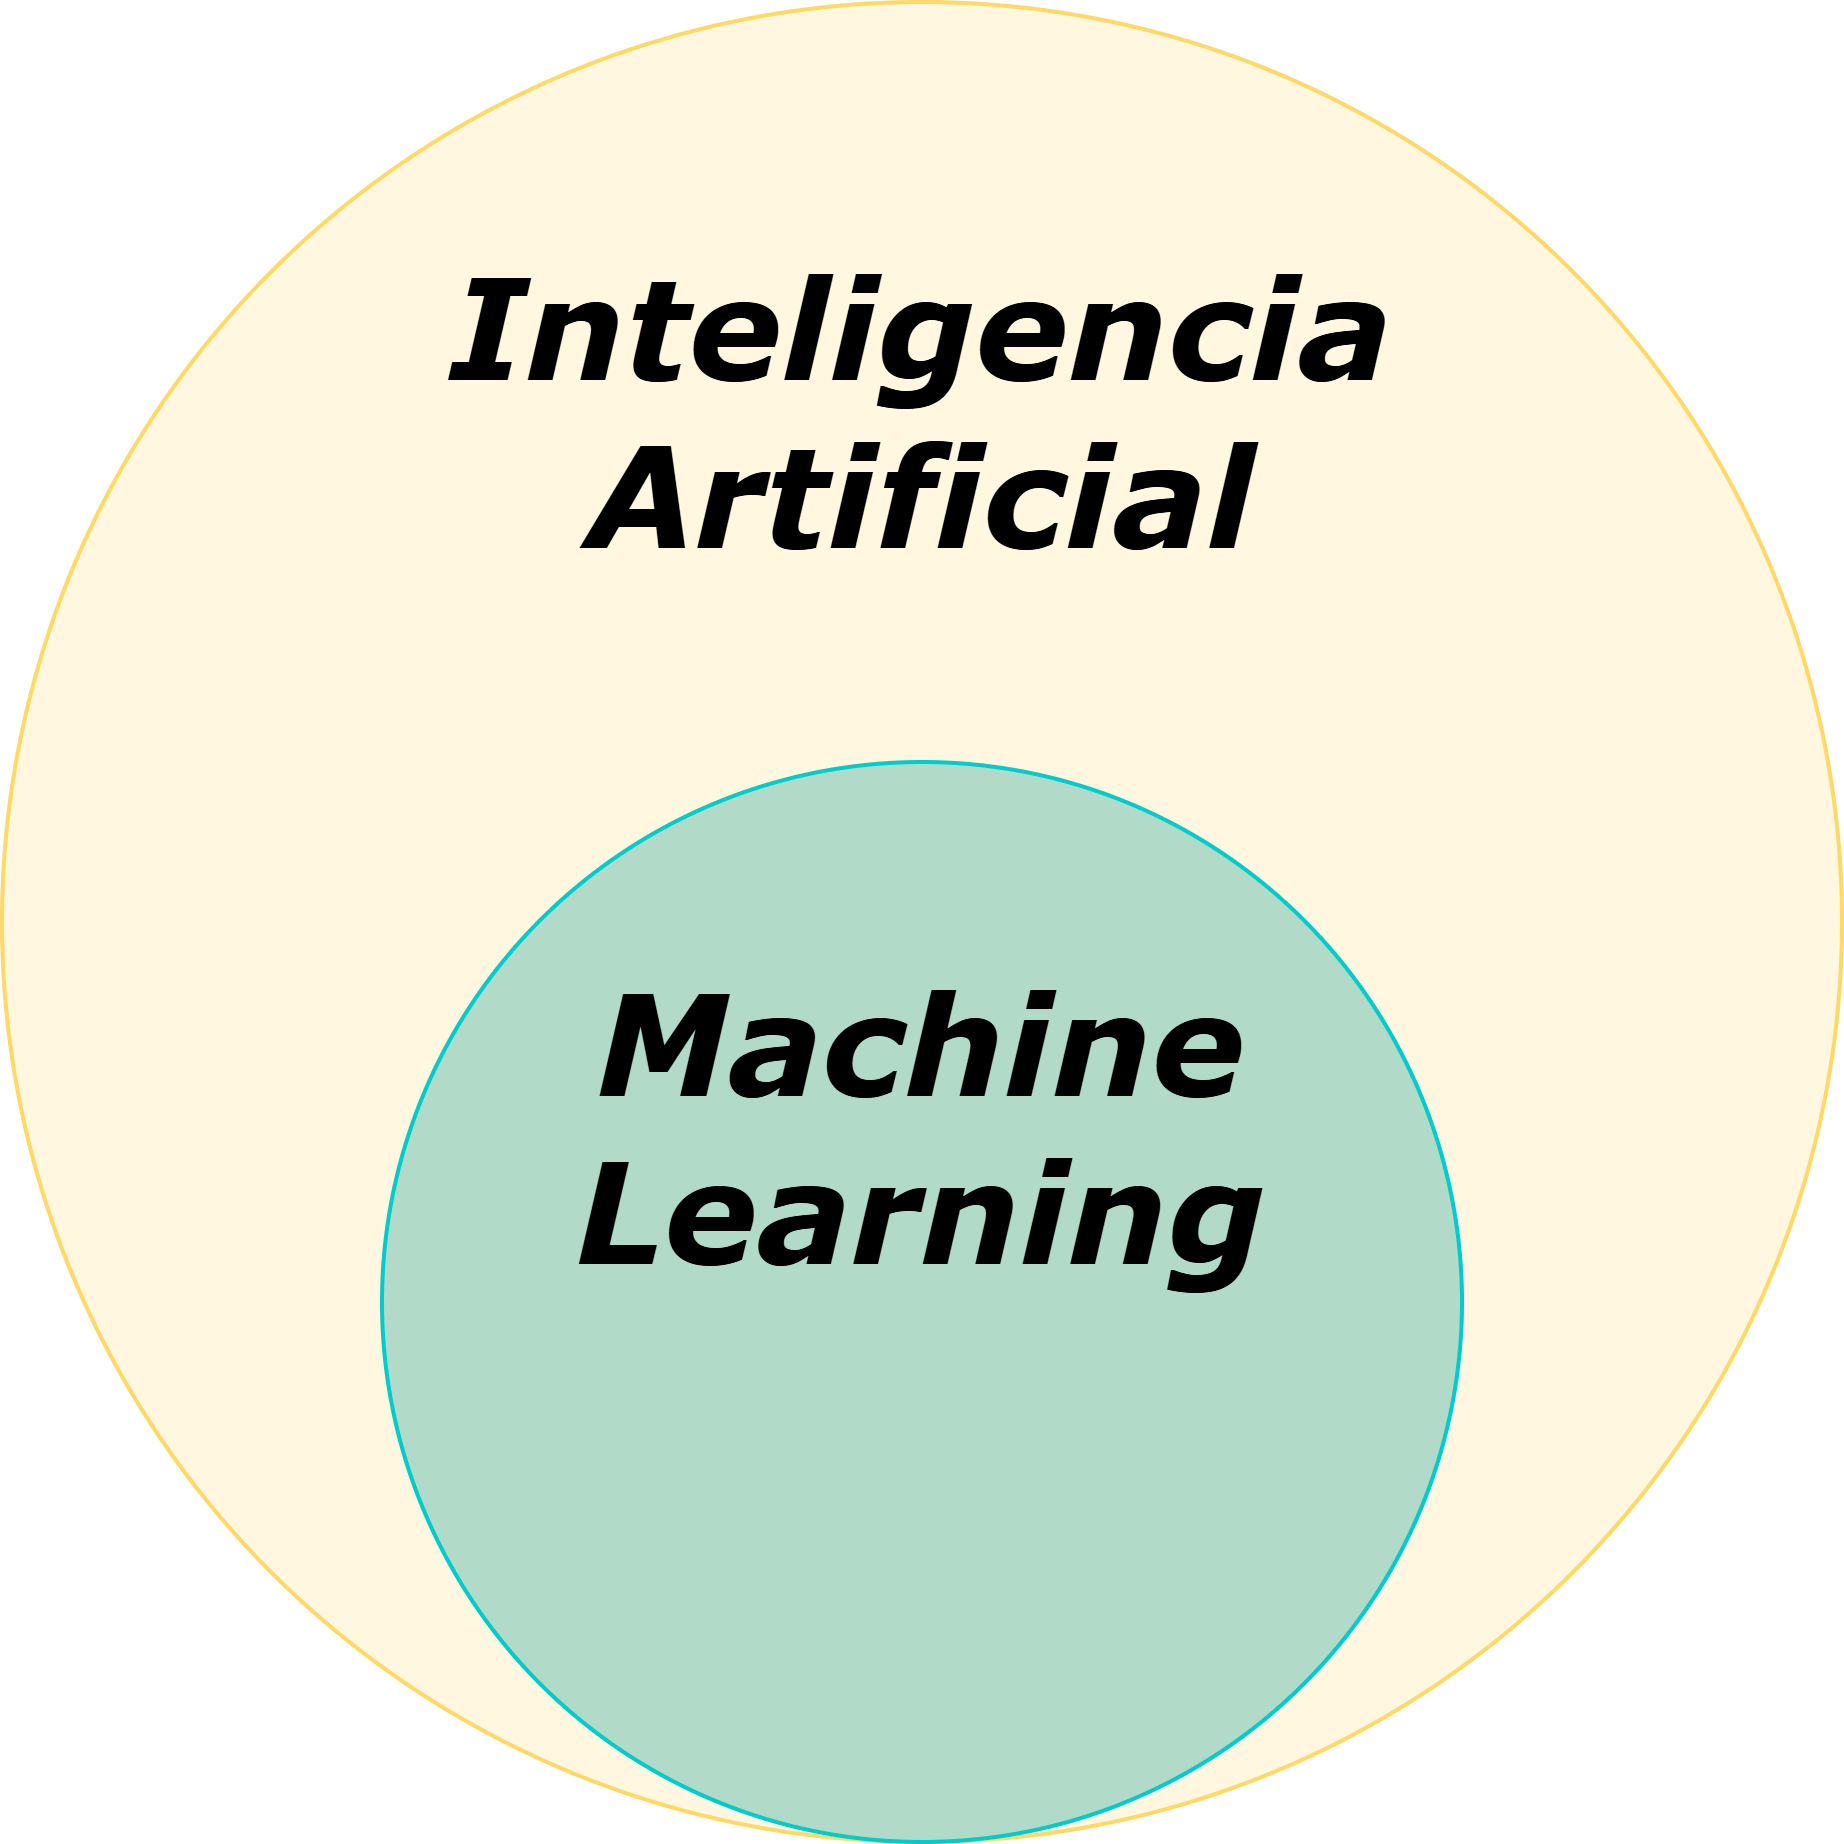
\includegraphics[width=\textwidth]{IA_ML.png}
    \end{column}

\end{columns}
\end{frame}

\begin{frame}{\LARGE Árboles de decisión}
    \begin{itemize}
        \item División del espacio de predictores.
        \item Determinar una predicción para cada región.
    \end{itemize}
    \vspace{1cm}

    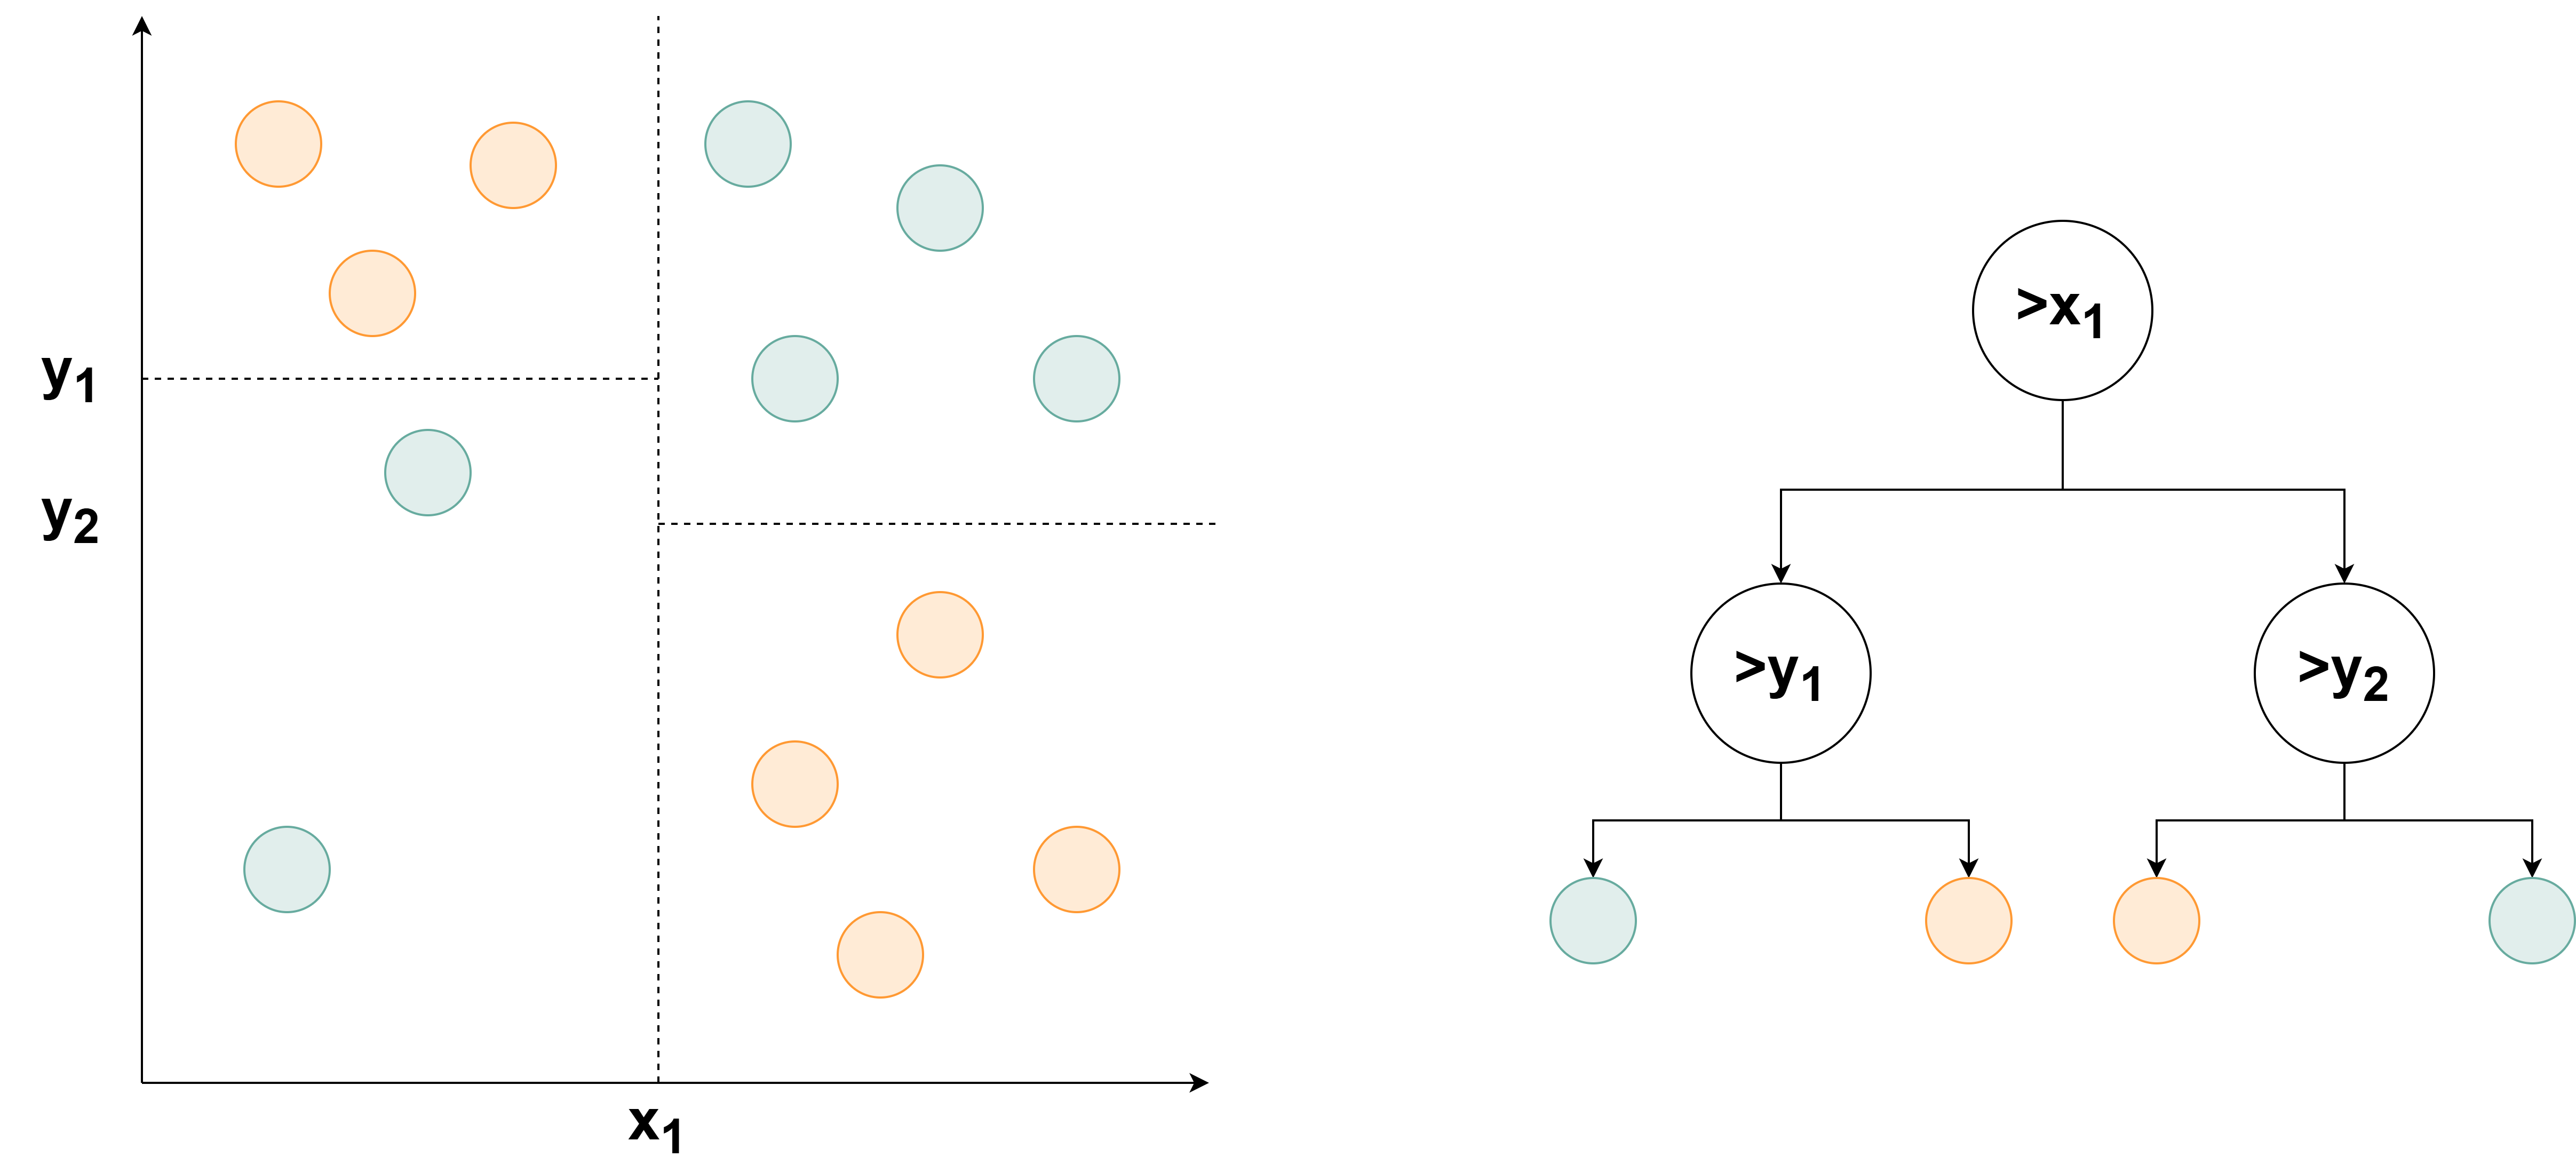
\includegraphics[width=\textwidth]{Arbol_De_Decision.png}
\end{frame}

\begin{frame}{\LARGE Árboles de decisión}
    \framesubtitle{Entrenamiento del árbol}
    \begin{itemize}
        \item \textit{Recursive binary splitting}
    \end{itemize}

    $Q_m$ conjunto de observaciones en el nodo $m$.\\
    Para cada cada posible división $\theta= (j,t_m.):$
    \begin{equation*}
        \begin{split}
            Q^{left}_m(\theta) &= \{ (X_i,Y_i)|x_{i_j} \leq t_m \} \\
            Q^{right}_m(\theta) &= \{ (X_i,Y_i)|x_{i_j} > t_m \}
        \end{split}
    \end{equation*}

    \begin{equation*}
        \mathcal{I}(Q_m,\theta)= \frac{|Q^{left}_m|}{|Q_m|}\mathcal{L}(Q^{left}_m(\theta))+\frac{|Q^{right}_m|}{|Q_m|}\mathcal{L}(Q^{right}_m(\theta))
    \end{equation*}

    $\mathcal{L}()$ función de impureza.
\end{frame}

\begin{frame}{\LARGE Árboles de decisión}
    \framesubtitle{Árboles de regresión}
    \begin{columns}[T]

        \begin{column}{0.45\textwidth}
            \textbf{Error cuadrático medio (MSE)}:
            \begin{equation*}
                \mathcal{L}(Q_m)=\frac{1}{|Q_m|}\sum_{y \in Q_m}(y-\bar{y}_m)^2
            \end{equation*}

            \begin{equation*}
                \bar{y}_m=\frac{1}{|Q_m|}\sum_{y \in Q_m}y
            \end{equation*}

        \end{column}

        \begin{column}{0.55\textwidth}
            \textbf{Error Medio absoluto (MAE)}:
            \begin{equation*}
                \mathcal{L}(Q_m)=\frac{1}{|Q_m|} \sum_{y \in Q_m} |y- mediana(y)_m|
            \end{equation*}

            \begin{equation*}
                mediana(y)_m=\underset{y \in Q_m}{mediana}(y)
            \end{equation*}
        \end{column}
    \end{columns}
\end{frame}

\begin{frame}{\LARGE Árboles de decisión}
    \framesubtitle{Evitar el \textit{overfitting}}
    \begin{columns}[T]
        \begin{column}{0.55\textwidth}
            \textbf{\textit{Early Stopping}}:
            \begin{itemize}
                \item nº mínimo para división.
                \item nº mínimo para nodo terminal.
                \item Profundidad máxima del árbol.
                \item nº máximo de nodos terminales.
                \item Reducción mínima del error.
            \end{itemize}
        \end{column}

        \begin{column}{0.45\textwidth}
            \textbf{\textit{Tree Pruning}}:
            \begin{itemize}
                \item Generar árboles grandes.
                \item Buscar subárbol óptimo.
                \item \textit{Minimal Cost-complexity pruning}.
            \end{itemize}
        \end{column}
    \end{columns}
\end{frame}

\begin{frame}{\LARGE Métodos de ensamble}
    \begin{itemize}
        \item Acoplamiento de modelos.
        \item Modelo débil: algo mejor que el azar.
        \item \textit{Stacking, Bagging, Boosting}.
    \end{itemize}
    
\end{frame}

\begin{frame}{\LARGE Métodos de ensamble}
    \framesubtitle{\textit{Stacking}}
    \begin{itemize}
        \item Modelos base distintos.
        \item \textit{Out-of-fold predictions} para entrenar \textit{meta-model}.
        \item \textit{Meta-model} computa la predicción final.
    \end{itemize}

    \vspace{1cm}

    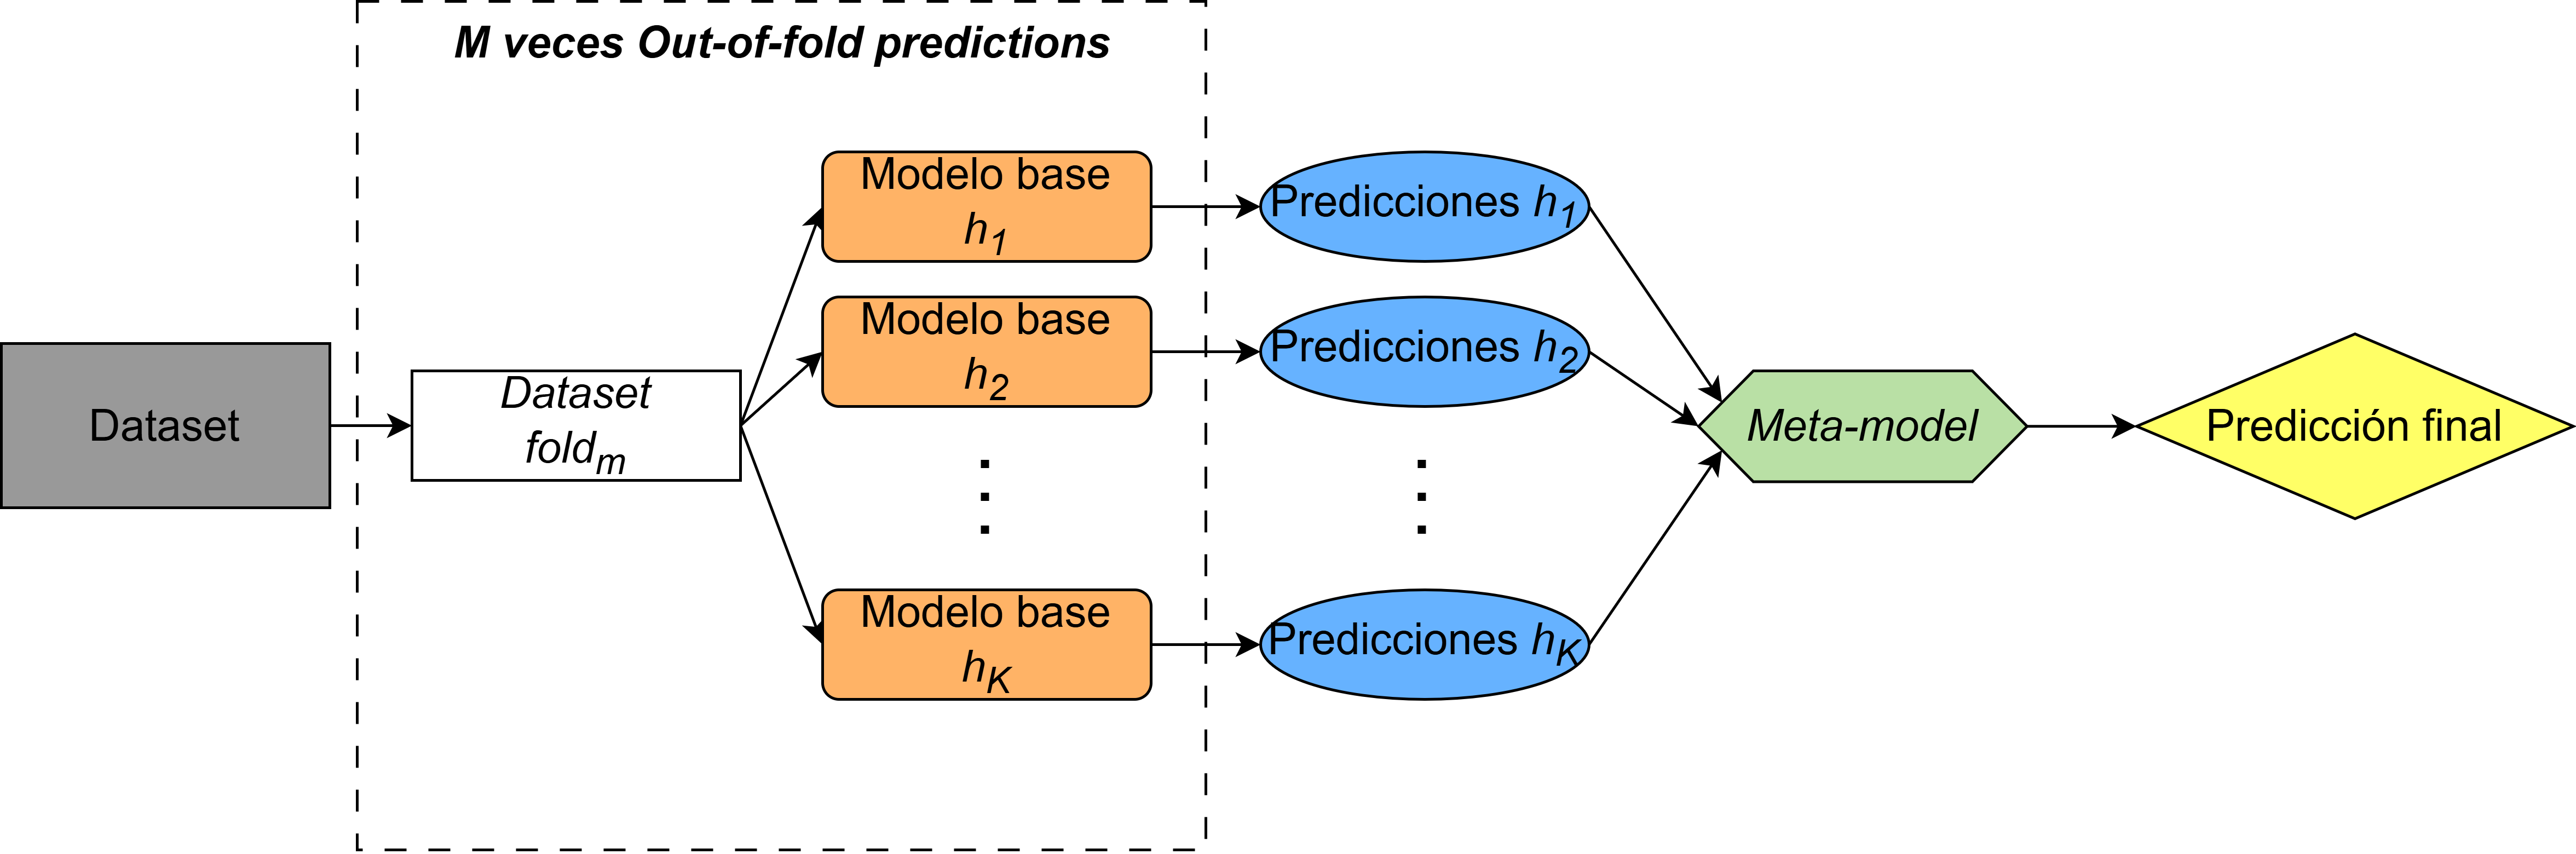
\includegraphics[width=\textwidth]{StackingDiagram.png}
\end{frame}

\begin{frame}{\LARGE Métodos de ensamble}
    \framesubtitle{\textit{Bagging}}
    \begin{itemize}
        \item Modelos base iguales.
        \item Entrenados sobre subconjuntos del conjunto de entrenamiento, obtenidos mediante remuestreo con remplazo \textit{(bootstrap)}.
        \item Predicciones finales obtenidas por agregación \textit{(aggregating)}.
    \end{itemize}

    \vspace{1cm}

    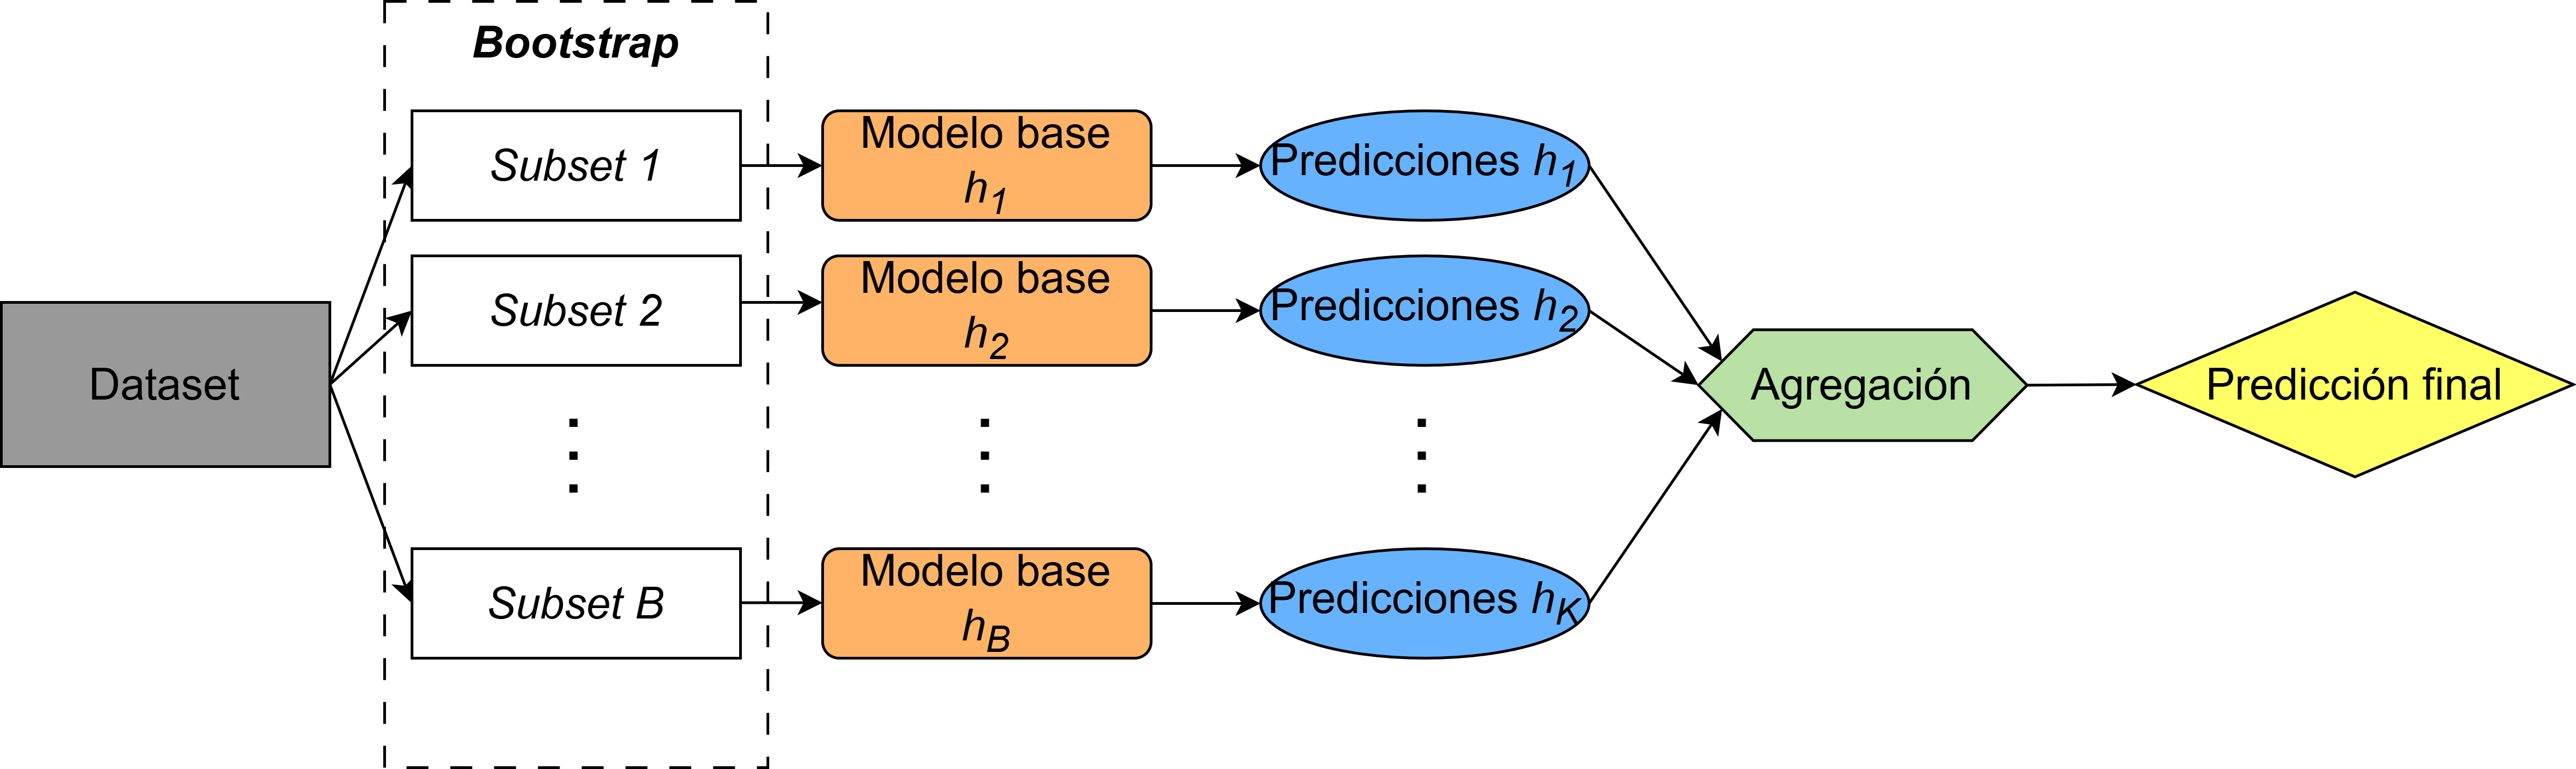
\includegraphics[width=\textwidth]{BaggingDiagram.png}
\end{frame}

\begin{frame}{\LARGE Métodos de ensamble}
    \framesubtitle{\textit{Bagging}}
    \textbf{Random Forest}
    \begin{itemize}
        \item Reducción de la correlación entre los árboles que componen el bosque.
        \item Para las divisiones de cada nodo, se tendrá en cuenta sólo un subconjunto aleatorio de características.
        \item Agregación final generaliza mejor a nuevos datos.
    \end{itemize}
\end{frame}

\begin{frame}{\LARGE Métodos de ensamble}
    \framesubtitle{\textit{Boosting}}
    \begin{itemize}
        \item Modelos base iguales.
        \item Entrenamiento secuencial y aditivo.
        \item Cada nuevo modelo base se entrena prestando mayor atención a las observaciones mal predichas por sus predecesores.
    \end{itemize}

    \vspace{1cm}

    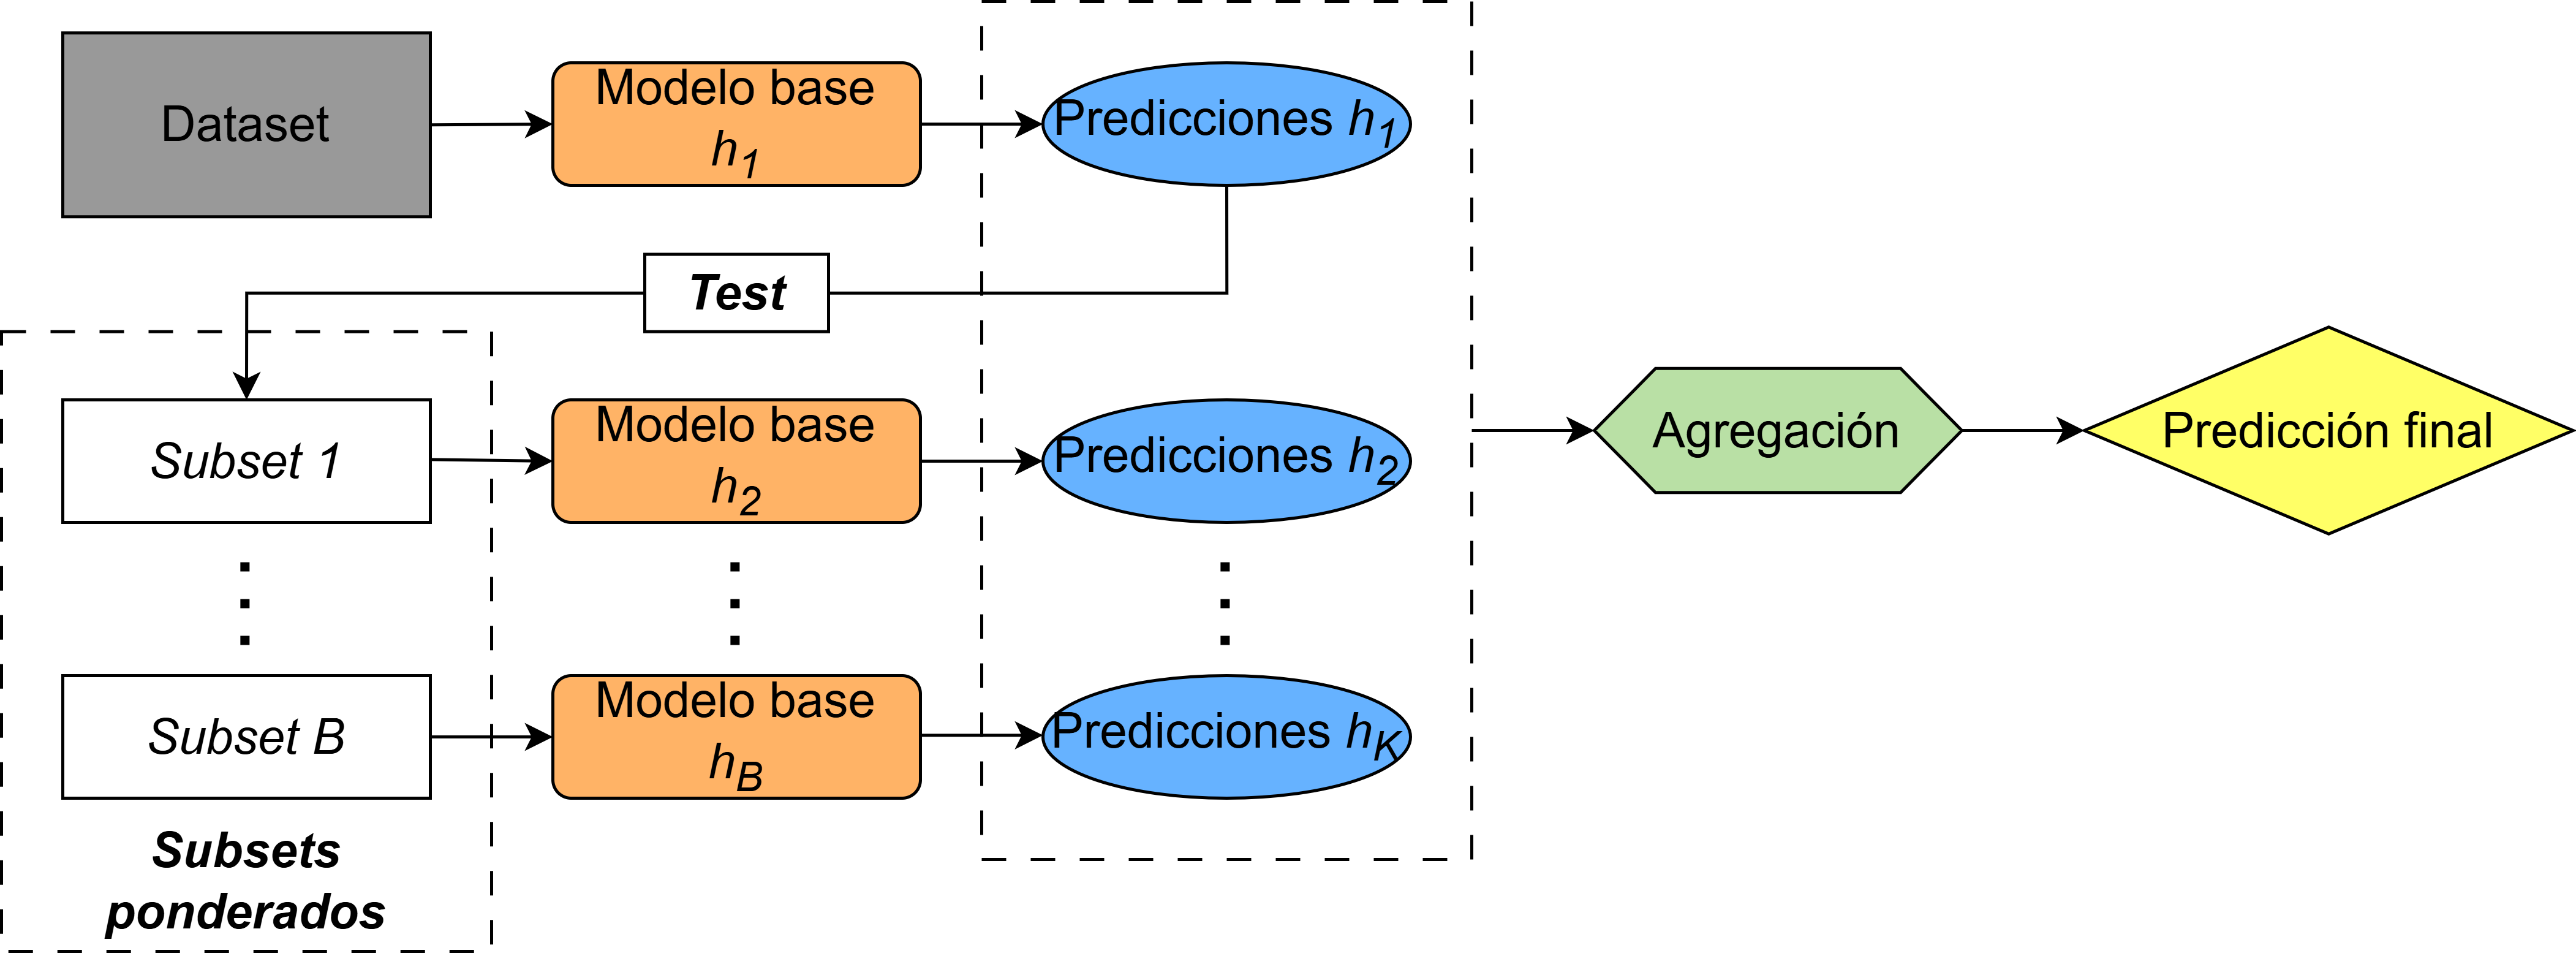
\includegraphics[width=\textwidth]{BoostingDiagram.png}
\end{frame}

\begin{frame}{\LARGE Métodos de ensamble}
    \framesubtitle{\textit{Boosting}}
    \begin{itemize}
        \item \textit{AdaBoost}: asignación de pesos a las muestras.
        \item \textit{Gradient Boosting}: los modelos base se entrenan para predecir el pseudoresiduo (gradiente negativo de la función pérdida).
        \item \textit{XGBoost (Xtreme Gradient Boosting)}: extiende el concepto de descenso del gradiente a la construcción del árbol \textit{(XGBTree)}.
    \end{itemize}
\end{frame}

\begin{frame}{\LARGE Estimación de la temperatura crítica}
    \framesubtitle{Introducción}
    \begin{itemize}
        \item Superconductores: materiales cuya resistividad eléctrica desaparece cuando se enfrían por debajo de su \textbf{temperatura crítica ($T_c$)}.
        \item Superconductores de alta temperatura.
        \item La predicción de la temperatura crítica es un problema abierto.
        \item Métodos de ensamble para predecir la temperatura crítica a partir de las propiedades físicas y químicas de los materiales.
    \end{itemize}
\end{frame}

\begin{frame}{\LARGE Estimación de la temperatura crítica}
    \framesubtitle{Conjuntos de datos y descriptores}
    \begin{itemize}
        \item Base de datos de materiales superconductores del \textit{Instituto Nacional para la Ciencia de Materiales (NIMS) de Japón}. 21.263 muestras de superconductores.
        \item Propiedades referidas a los elementos que componen el material:
    \end{itemize}
    \begin{columns}[T]
            \begin{column}{0.5\textwidth}
                \begin{itemize}
                    \item \textbf{Número de elementos}
                    \item \textbf{Masa atómica} $[UMA]$
                    \item \textbf{Primera energía de ionización} \textit{(fie)} $[kJ/mol]$
                    \item \textbf{Radio atómico} $[pm]$
                    \item \textbf{Densidad} $[kg/m^3]$
                \end{itemize}
            \end{column}

            \begin{column}{0.5\textwidth}
                \begin{itemize}
                    \item \textbf{Afinidad electrónica} $[kJ/mol]$
                    \item \textbf{Calor de fusión} $[kJ/mol]$
                    \item \textbf{Conductividad térmica} $[W/(m \cdot K)]$
                    \item \textbf{Valencia}
                \end{itemize}
            \end{column}
        \end{columns}
\end{frame}

\begin{frame}{\LARGE Estimación de la temperatura crítica}
    \framesubtitle{Conjuntos de datos y descriptores}
    \begin{itemize}
        \item Familias de descriptores estadísticos referentes a los compuestos:
    \end{itemize}
    \begin{columns}[T]
            \begin{column}{0.5\textwidth}
                \begin{itemize}
                    \item \textbf{Media aritmética} (mean\_*)
                    \item \textbf{Media ponderada} (wtd\_mean\_*)
                    \item \textbf{Media geométrica} (gmean\_*)
                    \item \textbf{Media geométrica ponderada} (wtd\_gmean\_*)
                    \item \textbf{Entropía} (entropy\_*)
                \end{itemize}
            \end{column}

            \begin{column}{0.5\textwidth}
                \begin{itemize}
                    \item \textbf{Entropía ponderada} (wtd\_entropy\_*)
                    \item \textbf{Rango} (range\_*)
                    \item \textbf{Rango ponderado} (wtd\_range\_*)
                    \item \textbf{Desviación estandar} (std\_*)
                    \item \textbf{Desviación estandar ponderada} (wtd\_std\_*)
                \end{itemize}
            \end{column}
        \end{columns}
\end{frame}

\begin{frame}{\LARGE Estimación de la temperatura crítica}
    \framesubtitle{Conjunto de datos y descriptores}
    Familias de descriptores para el YBCO:
    \begin{columns}[t]

% ===== Columna 1: Mean =====
\begin{column}{0.5\textwidth}
\begin{block}{Propiedades mean}
\begin{footnotesize}
\begin{tabular}{lr}
\hline
\textbf{Propiedad} & \textbf{Valor} \\
\hline
mean\_atomic\_mass & 68.24625 \\
mean\_fie & 886.18 \\
mean\_atomic\_radius & 147.4 \\
mean\_Density & 3389.3286 \\
mean\_ElectronAffinity & 131.89 \\
mean\_FusionHeat & 7.1844 \\
mean\_ThermalConductivity & 87.007096 \\
mean\_Valence & 2.8 \\
\hline
\end{tabular}
\end{footnotesize}
\end{block}
\end{column}

% ===== Columna 2: Range =====
\begin{column}{0.5\textwidth}
\begin{block}{Propiedades range}
\begin{footnotesize}
\begin{tabular}{lr}
\hline
\textbf{Propiedad} & \textbf{Valor} \\
\hline
range\_atomic\_mass & 121.3276 \\
range\_fie & 810.6 \\
range\_atomic\_radius & 205.0 \\
range\_Density & 8958.571 \\
range\_ElectronAffinity & 335.05 \\
range\_FusionHeat & 12.878 \\
range\_ThermalConductivity & 399.9911 \\
range\_Valence & 3.0 \\
\hline
\end{tabular}
\end{footnotesize}
\end{block}
\end{column}
\end{columns}
% ===== Columna 3: critical_temp =====

\centering
\begin{block}{Temperatura Crítica}
\begin{footnotesize}
\begin{tabular}{lr}
\hline
\textbf{Propiedad} & \textbf{Valor} \\
\hline
critical\_temp & 72.0 \\
\hline
\end{tabular}
\end{footnotesize}
\end{block}





\end{frame}


\begin{frame}{\LARGE Estimación de la temperatura crítica}
    \framesubtitle{Modelado}
    \begin{itemize}
        \item \textit{Random Forest}
        \item \textit{XGBoost}
        \item \textit{Árbol de decisión simple}
    \end{itemize}
    \vspace{1cm}
    \begin{itemize}
        \item Función de pérdida: Error cuadrático medio (MSE)
    \end{itemize}
\end{frame}

\begin{frame}{\LARGE Estimación de la temperatura crítica}
    \framesubtitle{Modelado}
    \textbf{Métricas de evaluación}
    \begin{columns}[T]
            \begin{column}{0.5\textwidth}
                \begin{itemize}
                    \item $RMSE=\sqrt{\sum_{i=1}^n \frac{(\hat{y}_i-y_i)^2}{n}}$ 
                \end{itemize}
            \end{column}

            \begin{column}{0.5\textwidth}
                \begin{itemize}
                    \item $R^2=1-\frac{\sum_{i=1}^n (y_i-\hat{y}_i)^2}{\sum_{i=1}^n (y_i-\bar{y}_i)^2}$
                \end{itemize}
            \end{column}
    \end{columns}
    \vspace{0.5cm}
    \begin{itemize}
        \item $MAPE=\frac{100}{n} \sum_{i=1}^n \left|\frac{\hat{y}_i-y_i}{y_i}\right| \, \rightarrow \, sMAPE=\frac{100}{n} \sum_{i=1}^n \left|\frac{\hat{y}_i-y_i}{(\hat{y}_i+y_i)/2}\right|$
    \end{itemize}

    \vspace{1cm}

    \textbf{Evaluación previa}
    \begin{itemize}
        \item Evaluación del rendimiento mediante \textit{cross-validation}.
    \end{itemize}
    \begin{table}[H]
        \centering
        \begin{tabular}{r|c|c|c}
                                & \textbf{$RMSE\,(K)$} & \textbf{$R^2$} & \textbf{$sMAPE\,(\%)$} \\ \hline
            \textbf{Random Forest} & 9.718           & 0.920          & 26.373           \\ \hline
            \textbf{XGBoost}       & 9.787           & 0.919          & 32.424           \\ \hline
            \textbf{Decision Tree} & 12.403          & 0.869          & 29.186          
        \end{tabular}
    \end{table}
\end{frame}

\begin{frame}{\LARGE Estimación de la temperatura crítica}
    \framesubtitle{Resultados}
    \begin{itemize}
        \item Entrenamiento sobre el subconjunto de entrenamiento.
        \item Validación sobre el subconjunto de test.
    \end{itemize}
    \begin{table}[H]
        \centering
        \begin{tabular}{r|c|c|c}
                                & \textbf{$RMSE\,(K)$} & \textbf{$R^2$} & \textbf{$sMAPE\,(\%)$} \\ \hline
            \textbf{Random Forest} & 9.042           & 0.929          & 25.187           \\ \hline
            \textbf{XGBoost}       & 8.973           & 0.925          & 32.975
        \end{tabular}
    \end{table}

    \begin{itemize}
    \item Tuneo de hiperparámetros.
    \end{itemize}

    \begin{table}[H]
        \centering
        \begin{tabular}{r|c|c|c}
                                & \textbf{$RMSE\,(K)$} & \textbf{$R^2$} & \textbf{$sMAPE\,(\%)$} \\ \hline
            \textbf{Random Forest} & 8.979           & 0.930          & 25.740           \\ \hline
            \textbf{XGBoost}       & 8.668           & 0.935          & 27.606
        \end{tabular}
    \end{table}
\end{frame}

\begin{frame}{\LARGE Estimación de la temperatura crítica}
    \framesubtitle{Resultados - Comparación entre los valores reales y predichos}
    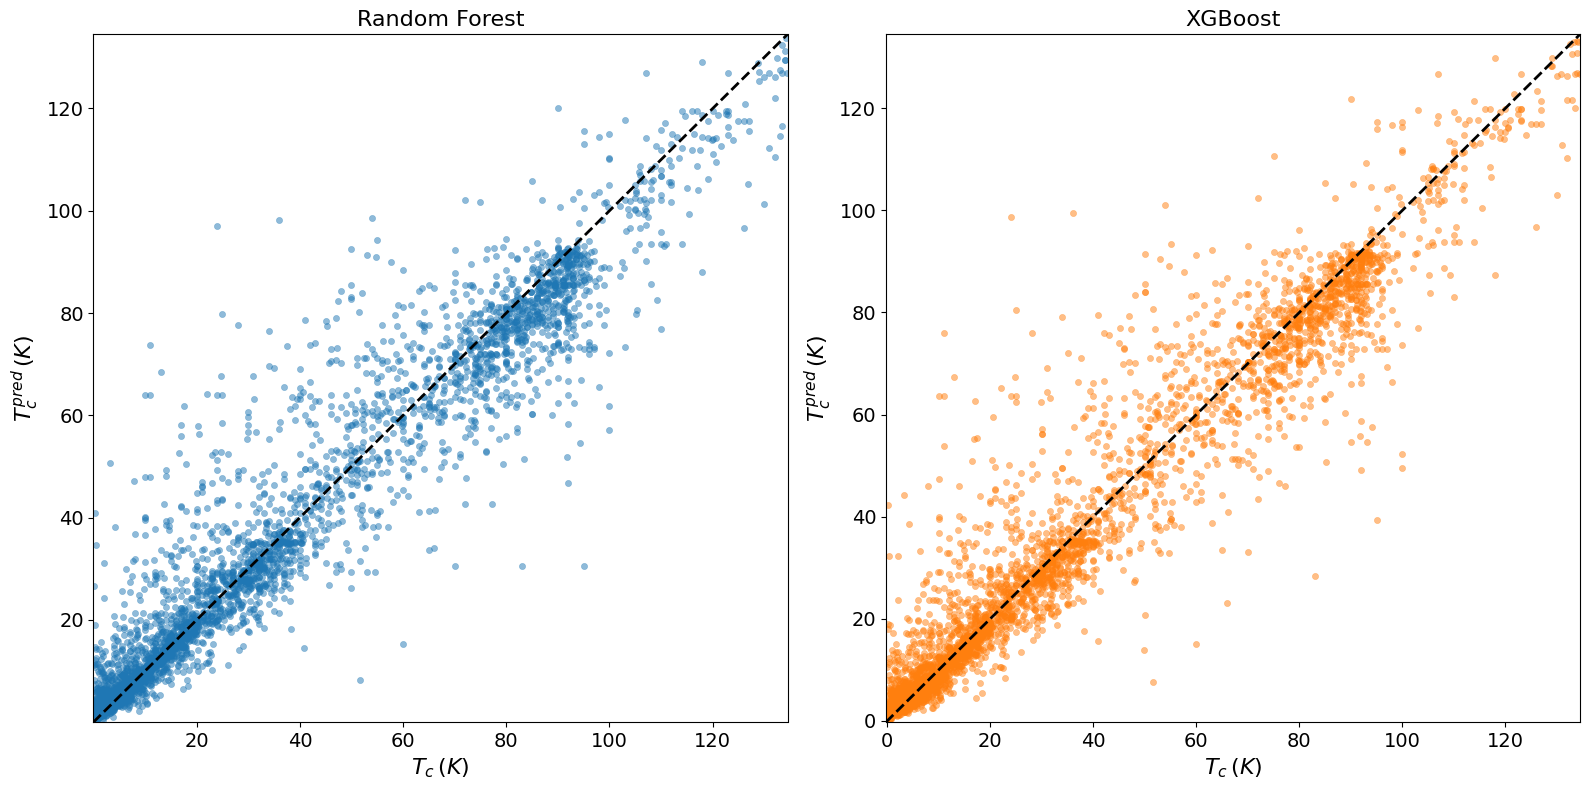
\includegraphics[width=\textwidth]{Real_Pred_1.png}
\end{frame}

\begin{frame}{\LARGE Estimación de la temperatura crítica}
    \framesubtitle{Resultados - Importancia de las variables}
    \includegraphics[width=\textwidth]{ImpVar_1.png}
\end{frame}

\begin{frame}{\LARGE Estimación de la temperatura crítica}
    \framesubtitle{Conclusiones}
    \begin{table}[H]
        \centering
        \begin{tabular}{r|c|c|c}
                                & \textbf{$RMSE\,(K)$} & \textbf{$R^2$} & \textbf{$sMAPE\,(\%)$} \\ \hline
            \textbf{Random Forest} & 8.979           & 0.930          & 25.740           \\ \hline
            \textbf{XGBoost}       & 8.668           & 0.935          & 27.606
        \end{tabular}
    \end{table}
    \includegraphics[width=\textwidth]{ImpVar_1.png}
\end{frame}

\begin{frame}{\LARGE Estimación de la temperatura crítica}
    \framesubtitle{Conclusiones}
    \begin{itemize}
        \item Capturan las tendencias globales.
        \item Limitados para predicciones individuales.
        \item Interpretabilidad: análisis de importancia de variables.
        \item Equilibrio entre precisión y explicabilidad.
    \end{itemize}
\end{frame}


\end{document}
